% =====================================================================
% A Pilot-Budget Benchmark for Passive RIS Phase Control
%
% Narrow benchmark paper. Every number is read from:
%   results/link_level_tier2/summary.json         (supplied-CSI study)
%   results/pilot_limited/summary.json            (M = 16, 64)
%   results/pilot_positive_control/summary.json   (M = 1025)
%   results/pilot_positive_control/observability_check.json
% Regenerate with the commands in docs/TIER2_CORRECTIONS.md.
% Per-result verdicts and reasoning: docs/RESULTS_REPORT.md
% =====================================================================
\documentclass[journal]{IEEEtran}
\IEEEoverridecommandlockouts

\usepackage{amsmath,amssymb,amsfonts}
\usepackage{graphicx}
\usepackage{booktabs}
\usepackage{url}
\usepackage{bm}
\usepackage{xspace}
\usepackage[hidelinks]{hyperref}

\graphicspath{{results/link_level_tier2/seed_42/}{results/tier01_report/}}

\newcommand{\dB}{\,dB\xspace}
\DeclareMathOperator{\atantwo}{atan2}

\begin{document}

\title{Separability, Acquisition Cost, and Estimator Limits\\ in Passive RIS Phase Control:\\ A Reproducible Pilot-Budget Benchmark}

\author{Anonymous Author(s)%
\thanks{Submitted for review. Affiliation withheld. Simulation code, result artifacts with input hash manifests, and a per-result audit are released with the paper.}}

\markboth{Manuscript for review}{Anonymous: A Pilot-Budget Benchmark for Passive RIS Phase Control}

\maketitle

%% ===================================================================
\begin{abstract}
Phase design for a reconfigurable intelligent surface (RIS) is routinely posed as an optimization problem and attacked with iterative, distributed or learned solvers. We show by measurement that for a single-antenna transmitter and receiver with supplied channel estimates the problem is \emph{separable}: the optimal phase of each element depends on that element's own cascaded coefficient and one globally shared scalar, so the closed-form solution is exact, element-local, and admits no improvement. On a contiguous 1024-element $32\times32$ aperture at 28\,GHz, the closed form and the perfect-CSI bound differ by $0.000\pm0.000$\dB over five independent seeds, while two iterative solvers finish 0.02--0.03\dB below it. The design question is therefore not optimization but \emph{acquisition}: a passive aperture has no receive chain, so the only channel information available is a small number of receiver-reported probe responses, and recovering $N+1=1025$ complex coefficients from $M\ll N$ measurements is rank-deficient. We contribute a reproducible benchmark for that problem in which every pilot symbol is charged, including the symbols spent acquiring training labels. Charging them reverses conclusions: exhaustive $N+1$-probe least squares attains the best channel knowledge by roughly ten decibels, yet after pilot overhead it only ties a 16-probe LMMSE estimator ($3.277\pm0.059$ against $3.251\pm0.056$\,bit/s/Hz) and is overtaken at $M=64$. We further introduce an \emph{observability certificate}: a noiseless algebraic round-trip that verifies a benchmark's features are sufficient before any inference claim is made. Ours confirms full rank and attains the oracle to ten decimal places in 32-bit arithmetic. We use it to scope, rather than assert, a negative finding about the learned predictors we evaluated. Aperture scaling is validated against the coherent-combining law to within 0.1\dB over a sixteen-fold increase in element count.
\end{abstract}

\begin{IEEEkeywords}
Reconfigurable intelligent surface, channel acquisition, pilot overhead, passive beamforming, benchmark, reproducibility.
\end{IEEEkeywords}

%% ===================================================================
\section{Introduction}
\label{sec:intro}
\IEEEPARstart{A}{reconfigurable} intelligent surface is a planar array of nearly passive elements whose reflection phases can be programmed to reshape propagation~\cite{direnzo2020,basar2019,wu2021tutorial}. At millimetre-wave frequencies, where blockage can remove tens of decibels from the direct path~\cite{rappaport2015}, a surface supplies an alternative reflected route whose coherent array gain grows as $O(N^2)$ in the element count~\cite{wu2019joint,bjornson2020}.

Most of the design literature treats phase selection as an optimization problem. Alternating optimization and semidefinite relaxation~\cite{wu2019joint,luo2010}, discrete-phase variants~\cite{wu2020discrete}, weighted sum-rate maximization by successive approximation~\cite{guo2020}, and energy-efficiency formulations~\cite{huang2019} all solve a program per coherence block. A parallel line amortizes that program into a learned forward pass, using deep reinforcement learning~\cite{huang2020drl}, compressive sensing with deep learning~\cite{taha2021}, or graph neural networks~\cite{shen2021gnn}. A further line distributes the learning itself, with devices or base stations as federated clients~\cite{elbir2022,mcmahan2017,kairouz2021}.

This paper makes a narrower and, we argue, prior claim. For the canonical single-user setting with supplied channel estimates the optimization problem is \emph{already solved in closed form, element by element}. Section~\ref{sec:sep} states the two-line argument and Section~\ref{sec:results} measures it: the closed form is indistinguishable from the perfect-CSI bound, and iterative solvers land marginally below it. Whatever a distributed or learned method contributes in that setting, it cannot be a better phase configuration.

The genuinely open problem sits one step earlier. A passive element is a patch of tunable impedance with no low-noise amplifier, mixer or converter --- adding $N$ receive chains would make it an antenna array and forfeit the cost argument that motivates surfaces in the first place. It follows that a tile cannot measure its own channel. What the system can do is apply $M$ known probing configurations while the transmitter sends pilots and have the \emph{receiver} report the responses~\cite{zheng2022survey,wang2020ce,he2020cascaded}. With $M<N+1$ the resulting linear system is rank-deficient, and no estimator resolves the nullspace without further assumptions. That is the problem a prior --- statistical or learned --- could legitimately address.

\textbf{Contributions.}
\begin{enumerate}
\item \textbf{A separability measurement (Section~\ref{sec:sep}, Table~\ref{tab:sep}).} On a contiguous 1024-element aperture, closed-form alignment and the perfect-CSI bound agree to $0.000\pm0.000$\dB over five seeds; projected gradient ascent and a surrogate maximizer finish $0.021\pm0.003$ and $0.032\pm0.003$\dB below. We state the boundary this places on distributed and learned phase design, and where the boundary moves.
\item \textbf{A pilot-budget benchmark with acquisition charged (Section~\ref{sec:bench}).} Six schemes are designed from exactly $M$ receiver-reported responses and scored on held-out true channels, with every pilot symbol charged --- including the $N+1$ orthogonal probes spent acquiring each training label. Charging them reverses the ranking of the best channel estimator.
\item \textbf{An observability certificate (Section~\ref{sec:cert}).} A noiseless algebraic round-trip that verifies, before any inference claim, that a benchmark's features are information-sufficient. Ours reports full rank, a relative reconstruction error of $3.2\times10^{-13}$, and attainment of the oracle in \emph{32-bit} arithmetic.
\item \textbf{A validated simulator and an explicitly scoped negative note (Sections~\ref{sec:model},~\ref{sec:disc}).} Aperture scaling matches the coherent-combining law to within 0.1\dB across a sixteen-fold element increase. The learned predictors we evaluated are reported as a limitation of a specific implementation, certified against the observability result, rather than as a claim about learning or federation.
\end{enumerate}

We deliberately do \emph{not} claim a novel phase-design method, a performance improvement over prior art, a circuit implementation, or a general statement about machine learning for RIS.

%% ===================================================================
\section{System and Observation Model}
\label{sec:model}

\subsection{One contiguous aperture}
A $32\times32$ uniform planar array is partitioned into a $4\times4$ grid of contiguous $8\times8$ tiles, giving $T=16$ tiles, $N_t=64$ elements per tile and $N=1024$ elements. At $f_c=28$\,GHz the half-wavelength pitch is $5.36$\,mm and the cell-edge aperture is $0.1714\times0.1714$\,m. The surface centre is $(5,0,1.5)$\,m on the $y=0$ wall, the transmitter is at $(5,10,1.5)$\,m, and receivers are uniform in $[0.5,9.5]\times[1,9.5]\times[1,2]$\,m.

Channels are generated over the \emph{whole} aperture per scene and then sliced into tiles, so all tiles share one scattering realization and their contributions combine coherently by construction. Line-of-sight phases use exact transmitter--element and element--receiver distances: the Fraunhofer distance of this aperture is $2D^2/\lambda\approx11$\,m and receivers lie inside a 10\,m room, so a planar steering approximation would be inappropriate. Each hop carries five non-line-of-sight plane waves with directions drawn in the half-space in front of the panel and exponentially decaying complex gains; spatial correlation therefore arises from path geometry rather than from an imposed correlation matrix~\cite{bjornson2021rayleigh}. Close-in path loss is $\mathrm{PL}(d)=(\lambda/4\pi)^2 d^{-\alpha}$ with $\alpha=2.5$ per reflecting hop and $\alpha=3.5$ on the direct link, the Rician factor is 10\dB, each element contributes an aperture factor $G_e=4\pi(\lambda/2)^2/\lambda^2=\pi$ per hop~\cite{tang2021}, and the direct link carries 30\dB of excess blockage loss.

This is a synthetic propagation model, not a calibrated electromagnetic or ray-traced one~\cite{alkhateeb2019}. Mutual coupling, angle-dependent element patterns and intra-block receiver mobility are omitted. The physical panel size does not imply a silicon die size.

\subsection{Effective channel}
With unit-modulus reflection, for tile $t$ and element $n$ with cascaded coefficient $c_{t,n}$,
\begin{equation}
h_{\mathrm{eff}}(\bm{\theta}) = h_{\mathrm{d}} + \sum_{t=1}^{T}\sum_{n=1}^{N_t} c_{t,n}\,e^{j\theta_{t,n}},
\qquad
\gamma = \rho\,\bigl|h_{\mathrm{eff}}(\bm{\theta})\bigr|^{2},
\label{eq:heff}
\end{equation}
where $h_{\mathrm{d}}$ is the blocked direct channel and $\rho=P_{\mathrm{t}}/\sigma^2$. The noise power is $-90$\,dBm and the operating point is $P_{\mathrm{t}}=30$\,dBm, so $10\log_{10}\rho=120$\dB. We note explicitly that $\rho$ is a transmit-to-noise ratio \emph{before} propagation and is not a received SNR; all reported SNRs are received.

\subsection{Limited-pilot passive acquisition}
\label{sec:obs}
The aperture applies known phase patterns $\phi_{m,n}$ while the transmitter sends pilots. The receiver measures and feeds back
\begin{equation}
y_m = h_{\mathrm{d}} + \sum_{n=1}^{N} c_n e^{j\phi_{m,n}} + w_m,
\qquad w_m\sim\mathcal{CN}(0,1/\rho),
\label{eq:pilot}
\end{equation}
normalized by the transmitted pilot amplitude. With $\bm{x}=[h_{\mathrm{d}},c_1,\dots,c_N]^{\!\top}$ and $\bm{A}_{m,:}=[1,e^{j\phi_{m,1}},\dots,e^{j\phi_{m,N}}]$ this is $\bm{y}=\bm{A}\bm{x}+\bm{w}$ with $\bm{A}\in\mathbb{C}^{M\times(N+1)}$. The probe codebook is a fixed seeded random design, so every probe illuminates every element and each measurement carries information about the whole channel.

For $M<N+1$ the matrix $\bm{A}$ has a nontrivial nullspace: infinitely many channel vectors explain the same measurements exactly. This is a rank deficiency, not a noise limitation, and it persists at arbitrarily high SNR. It is the structural reason a prior over channels could help, and it is the problem this benchmark poses.

%% ===================================================================
\section{Separability and What It Rules Out}
\label{sec:sep}

For any phase vector, the triangle inequality applied to~\eqref{eq:heff} gives
\begin{equation}
\bigl|h_{\mathrm{eff}}(\bm{\theta})\bigr| \;\le\; |h_{\mathrm{d}}| + \sum_{t,n}\bigl|c_{t,n}e^{j\theta_{t,n}}\bigr| \;=\; |h_{\mathrm{d}}| + \sum_{t,n}|c_{t,n}|,
\label{eq:bound}
\end{equation}
where the last step uses the fact that a unit-modulus phase shifter cannot alter magnitude, so the bound is independent of $\bm{\theta}$. Equality holds exactly when every term shares a common argument; choosing that of $h_{\mathrm{d}}$,
\begin{equation}
\theta^{\star}_{t,n} = \angle h_{\mathrm{d}} - \angle c_{t,n},
\label{eq:mrc}
\end{equation}
which attains~\eqref{eq:bound}. Because $\log_2(1+\rho|\cdot|^2)$ is monotone, \eqref{eq:mrc} also maximizes rate. If $h_{\mathrm{d}}=0$ any common reference suffices.

Three consequences follow, and they are the reason this paper is structured as it is.

\emph{The solution is exact.} Equation~\eqref{eq:mrc} is not a relaxation, a bound or an initialization. It attains the supremum, so no iterative or learned method can exceed it.

\emph{The solution is element-local.} $\theta^{\star}_{t,n}$ depends on $c_{t,n}$ and on the single scalar $\angle h_{\mathrm{d}}$ shared by all elements. There is no inter-element coupling, hence none between tiles, hence nothing for a distributed algorithm to exchange beyond one common phase reference.

\emph{The deployable rule is the plug-in rule.} With estimates $\hat{\bm{x}}$, $\hat\theta_{t,n}=\angle\hat h_{\mathrm{d}}-\angle\hat c_{t,n}$ maximizes the estimated-channel objective. It is not necessarily Bayes-optimal under estimation uncertainty --- a gap we measure rather than assume in Section~\ref{sec:results}.

It is worth being precise about what this does \emph{not} rule out, since the boundary is the useful part. Separability is a property of the single-user, single-antenna objective. With multiple users, interference couples the elements through the shared $h_{\mathrm{eff}}$ and the objective ceases to decompose~\cite{guo2020,huang2020drl}. And separability of the \emph{objective} does not imply separability of the \emph{inference}: under~\eqref{eq:pilot} with $M<N+1$, the estimate of any one coefficient depends jointly on all measurements. Distributed and learned design remain well-motivated in both regimes. They are not motivated in the regime most commonly used to evaluate them.

%% ===================================================================
\section{Benchmark Design}
\label{sec:bench}

\subsection{Schemes, at equal observations}
All equal-budget schemes receive exactly the same $M$ noisy complex responses and the same fixed codebook.

\begin{itemize}
\item \textbf{Best observed probe.} Re-apply $\bm{\phi}_{m^\star}$ with $m^\star=\arg\max_m|y_m|$. No channel model, no training; feedback is one index. The classical low-overhead floor.
\item \textbf{LMMSE followed by alignment.} With mean $\bm{\mu}$ and covariance $\bm{R}$ estimated from the training scenes,
\begin{equation}
\hat{\bm{x}} = \bm{\mu} + \bm{R}\bm{A}^{\mathsf{H}}\bigl(\bm{A}\bm{R}\bm{A}^{\mathsf{H}} + \rho^{-1}\bm{I}\bigr)^{-1}(\bm{y}-\bm{A}\bm{\mu}),
\label{eq:lmmse}
\end{equation}
with light diagonal loading, followed by~\eqref{eq:mrc}. This is the strongest linear use of a learned prior at the given budget~\cite{kay1993}, and therefore the control that any nonlinear prior must beat to justify itself.
\item \textbf{Local linear estimator followed by alignment.} Each tile independently ridge-regresses its own $(N_t{+}1)$ coefficients on the shared feedback, $\bm{W}_t=(\bm{Y}^{\mathsf{H}}\bm{Y}/S+\delta\bm{I})^{-1}\bm{Y}^{\mathsf{H}}\bm{X}_t/S$, with $\delta$ relative to input covariance power. No other tile's labels and no aggregation rounds are required. This is the decisive control for any distributed proposal.
\item \textbf{Full-probe least squares followed by alignment.} $N+1$ orthogonal DFT probes give per-coefficient variance $1/[\rho(N{+}1)]$. A deliberately higher-acquisition-cost control, kept distinct from the equal-$M$ schemes.
\item \textbf{Perfect-CSI alignment.} An unattainable-information reference. Its zero charged acquisition cost must not be read as a deployable operating point.
\item \textbf{No RIS} and \textbf{random phases}, as floors.
\end{itemize}

\subsection{Training labels are acquired, not given}
Priors must be fitted from something. We do not use simulator truth. For each of $S$ training and $V$ validation scenes the system spends its $M$ feedback probes \emph{and} a separate $N+1$ orthogonal DFT sequence to obtain a noisy channel label, for a training-data acquisition cost of $(S+V)(M+N+1)$ pilot symbols. Labels are finite-SNR least-squares estimates. True channels are reserved for scoring held-out scenes and for the explicitly labelled oracle. This is a substantial offline assumption and we state it as one.

\subsection{Charging for pilots}
Symbols spent probing are symbols not spent on data. The headline metric is therefore
\begin{equation}
R_{\mathrm{net}} = \max\Bigl\{0,\,1-\tfrac{M_{\mathrm{used}}}{L}\Bigr\}\;\mathbb{E}\bigl[\log_2(1+\gamma)\bigr],
\qquad L=2048,
\label{eq:netrate}
\end{equation}
with $M_{\mathrm{used}}=N+1$ for full-probe least squares and $M$ otherwise. Feedback latency, feedback errors, training amortization and controller computation are \emph{not} folded into~\eqref{eq:netrate}; their payloads are accounted separately in the released artifacts. We also report received SNR and fraction of oracle power, so that a scheme cannot appear robust merely by starting low.

\subsection{Protocol}
Each run uses $S=600$ training, $V=200$ validation and 600 test scenes, with seeds $\{42,123,456,789,1024\}$ and a fixed codebook seed. Every scheme is scored on the same held-out true channels within a seed. Confidence intervals are 95\% Student-$t$ with the seed as the independent unit; paired differences use matched seeds. Intervals do not quantify variation over codebook design or propagation model.

%% ===================================================================
\section{The Observability Certificate}
\label{sec:cert}

Benchmarks that feed engineered features to an estimator carry a failure mode that is rarely tested: the features may not retain the information the task requires, in which case every number measured on them describes the pipeline rather than the method. We propose a cheap check and report it as part of the benchmark.

Fix $M=N+1$, so that~\eqref{eq:pilot} is nominally determined, and evaluate the noiseless algebraic round-trip: form $\bm{A}$ from the deployed codebook, invert it, apply~\eqref{eq:mrc} to the recovered $\hat{\bm{x}}$, and score the resulting configuration on the true channel through the \emph{same} feature construction, normalization and phase-application path the estimators use.

For our codebook and geometry, $\bm{A}$ has full rank 1025 with condition number $9.4\times10^{3}$; the relative channel reconstruction error is $3.2\times10^{-13}$; and the recovered configuration attains fraction of oracle power $1.0000000010$ in double precision and $1.0000000002$ in \emph{single} precision. The single-precision result matters because it is the arithmetic the learned estimators use, so finite precision is excluded as an explanation for any shortfall.

The certificate supports two distinct uses. Positively, it establishes that the observation model, feature construction and application path are information-preserving, so a method evaluated here is evaluated against a sufficient input. Negatively, it converts an unexplained shortfall into a localized one: a method that underperforms on certified-sufficient features has an internal defect, and the benchmark can say so without speculating. We use it in exactly that way in Section~\ref{sec:disc}.

%% ===================================================================
\section{Results}
\label{sec:results}

\subsection{Aperture validation}
Coherent combination of $N$ comparable terms must scale received power as $N^2$, i.e.\ $20\log_{10}(1024/64)=24.08$\dB from 64 to 1024 elements. Measured reflected-only oracle gain over that range is 23.99--24.13\dB across the five seeds, and the per-element channel power spreads by only 0.06--0.18\dB across the surface. Fig.~\ref{fig:scaling} plots the curve against the law. We present this as validation rather than as a finding: its purpose is to establish that the simulator reproduces a closed-form physical result before any comparative claim is read from it.

\begin{figure}[!t]
\centering

\includegraphics[width=\columnwidth]{fig6_array_scaling}
\caption{Aperture scaling against the coherent-combining law. The reference line is anchored on reflected-only oracle power with the direct path excluded, so that direct-path dominance at small $N$ cannot produce an apparent departure from the law.}
\label{fig:scaling}
\end{figure}

\subsection{Separability, measured}
Table~\ref{tab:sep} reports supplied-CSI channel power gain and paired differences against the closed form. The closed form and the perfect-CSI bound are identical with a zero-width interval, as~\eqref{eq:mrc} requires. Both iterative solvers finish marginally \emph{below} it, with paired intervals a few thousandths of a decibel wide. The surface itself is worth $14.28\pm0.65$\dB relative to the blocked link; the choice among the four channel-aware designs is worth nothing.

\begin{table}[!t]
\centering
\caption{Supplied-CSI diagnostic: channel power gain and paired difference against closed-form alignment. Five seeds, 95\% Student-$t$ intervals.}
\label{tab:sep}
\renewcommand{\arraystretch}{1.15}
\setlength{\tabcolsep}{4pt}
\footnotesize
\begin{tabular}{@{}lrr@{}}
\toprule
\textbf{Scheme} & \textbf{Gain (dB)} & \textbf{Paired gap (dB)} \\
\midrule
Perfect-CSI bound            & $-92.328\pm0.311$  & $\phantom{-}0.000\pm0.000$ \\
Closed-form alignment, Eq.~\eqref{eq:mrc} & $-92.328\pm0.311$ & $\phantom{-}0.000\pm0.000$ \\
Projected gradient ascent    & $-92.349\pm0.311$  & $-0.021\pm0.003$ \\
Surrogate maximizer          & $-92.360\pm0.310$  & $-0.032\pm0.003$ \\
Random phases                & $-106.496\pm0.800$ & $-14.167\pm0.637$ \\
No RIS (blocked)             & $-106.613\pm0.811$ & $-14.284\pm0.647$ \\
\bottomrule
\end{tabular}
\end{table}

\subsection{Robustness of the plug-in rule}
Supplying estimates with normalized error power $\epsilon$ and scoring on true channels, the closed form retains $25.72$\dB of received SNR at $\epsilon=1$ against $27.67$\dB at $\epsilon=0$: a loss of 1.95\dB out of a 14.28\dB gain when error power equals signal power. The mechanism is aperture averaging --- a per-element estimate error mis-rotates a contribution carrying $O(1/N)$ of the total amplitude, and such errors do not compound. We report absolute SNR rather than relative degradation, because a scheme operating further from the optimum necessarily degrades less and a relative metric would reward that.

\subsection{Pilot-budget benchmark}
Table~\ref{tab:pilot} reports the benchmark at $M\in\{16,64\}$ and, for the determined case, $M=N+1=1025$. Fig.~\ref{fig:pilot} shows the $M=16$ comparison with seed-level intervals.

\begin{table*}[!t]
\centering
\caption{Pilot-budget benchmark. Five seeds at $M=16,64$; three at $M=1025$. 95\% Student-$t$ intervals. $R_{\mathrm{net}}$ from Eq.~\eqref{eq:netrate} with $L=2048$. ``Frac.\ oracle'' is the fraction of perfect-CSI received power.}
\label{tab:pilot}
\renewcommand{\arraystretch}{1.15}
\setlength{\tabcolsep}{5pt}
\footnotesize
\begin{tabular}{@{}lrrrrrrrrr@{}}
\toprule
& \multicolumn{3}{c}{$M=16$} & \multicolumn{3}{c}{$M=64$} & \multicolumn{3}{c}{$M=1025$ (determined)} \\
\cmidrule(lr){2-4}\cmidrule(lr){5-7}\cmidrule(lr){8-10}
\textbf{Scheme} & \textbf{SNR (dB)} & \textbf{$R_{\mathrm{net}}$} & \textbf{Frac.} & \textbf{SNR (dB)} & \textbf{$R_{\mathrm{net}}$} & \textbf{Frac.} & \textbf{SNR (dB)} & \textbf{$R_{\mathrm{net}}$} & \textbf{Frac.} \\
\midrule
Perfect CSI \emph{(not deployable)} & 27.67 & $8.388\pm0.078$ & 1.000 & 27.67 & $8.388\pm0.078$ & 1.000 & 27.84 & $8.419\pm0.110$ & 1.000 \\
\midrule
Full-probe LS \emph{(1025 probes)} & 25.18 & $3.277\pm0.059$ & 0.316 & 25.18 & $3.277\pm0.059$ & 0.316 & 25.44 & $3.300\pm0.084$ & 0.320 \\
LMMSE, Eq.~\eqref{eq:lmmse}        & 14.62 & $\bm{3.251\pm0.056}$ & 0.058 & 16.34 & $\bm{3.984\pm0.127}$ & 0.077 & 23.11 & $3.166\pm0.107$ & 0.253 \\
Local linear, per tile             & 14.36 & $3.022\pm0.055$ & 0.056 & 15.56 & $3.566\pm0.132$ & 0.069 & 17.87 & $2.282\pm0.117$ & 0.096 \\
Best observed probe                & 13.77 & $2.649\pm0.056$ & 0.049 & 13.91 & $2.727\pm0.039$ & 0.051 & 14.41 & $1.505\pm0.041$ & 0.053 \\
\midrule
No RIS (blocked)                   & 13.39 & $2.060\pm0.065$ & 0.045 & 13.39 & $2.060\pm0.065$ & 0.045 & 13.71 & $2.032\pm0.113$ & 0.045 \\
\bottomrule
\end{tabular}
\end{table*}

\begin{figure}[!t]
\centering
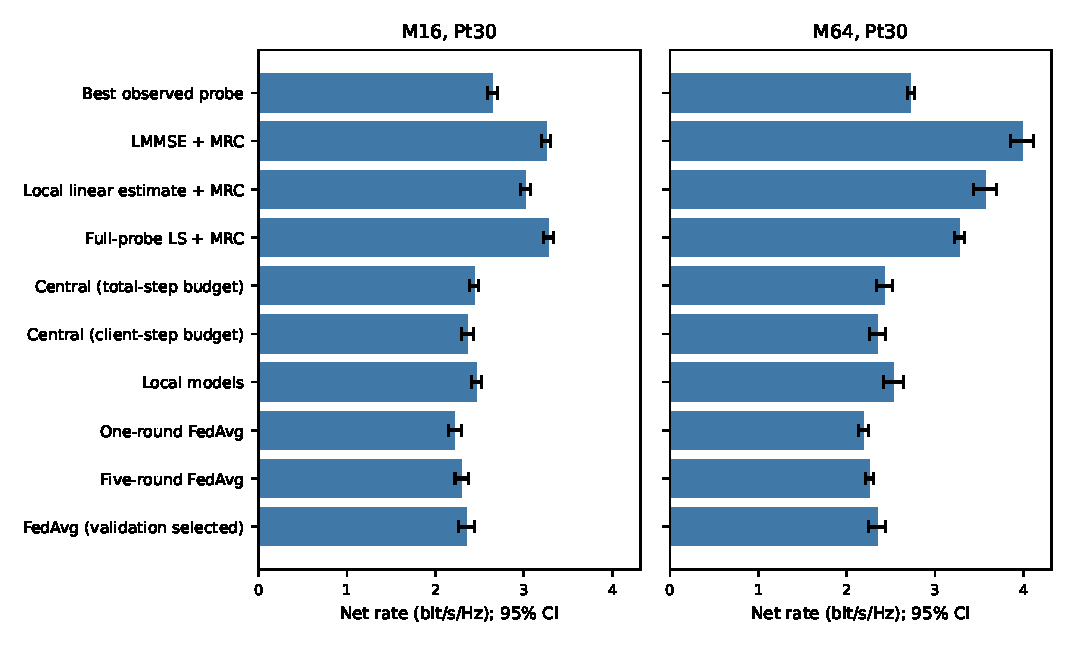
\includegraphics[width=\columnwidth]{pilot_comparison}
\caption{Pilot-adjusted rate at equal observations with seed-level 95\% intervals. Full-probe least squares uses 1025 probes and is plotted for reference; perfect CSI is excluded from the deployable comparison.}
\label{fig:pilot}
\end{figure}

Three findings follow.

\emph{The acquisition problem is the binding constraint.} At $M=16$ the best deployable scheme reaches under six per cent of the oracle's received power. At $M=1025$, where the system is determined, the best reaches under a third --- limited now by pilot noise rather than by rank. The gap to perfect CSI is therefore large and irreducible at realistic budgets, which is what makes the problem worth posing.

\emph{Estimators use information; the ranking is physically sensible.} Quadrupling the budget from 16 to 64 improves LMMSE by $0.733$ and the per-tile regression by $0.544$\,bit/s/Hz, while probe selection improves by $0.078$ --- exactly what a scheme that merely takes a maximum over a longer list should gain. A benchmark must demonstrate this kind of monotone, mechanism-consistent response before comparative claims made on it are credible.

\emph{Charging for pilots reverses the conclusion.} Full-probe least squares attains the best channel knowledge by a wide margin: roughly ten decibels of received SNR beyond the equal-$M$ schemes, and 0.32 of oracle power against 0.06. Charged for the half of every coherence block it consumes, it merely ties 16-probe LMMSE ($3.277\pm0.059$ against $3.251\pm0.056$, intervals overlapping) and is clearly overtaken at $M=64$ ($3.277$ against $3.984\pm0.127$). Reported on received SNR alone, exhaustive probing dominates and would be recommended; charged honestly, it does not. The crossover between purchasing channel knowledge and retaining the block for data lies between 16 and 1025 probes, and by $M=64$ a statistical estimator is already past the point where exhaustive probing repays its overhead. This is the benchmark's principal quantitative result and it exists only because acquisition is charged.

%% ===================================================================
\section{Discussion, Scope and Limitations}
\label{sec:disc}

\textbf{What the separability result is and is not.} It is a statement about the single-user, single-antenna objective with supplied estimates, and in that regime it is decisive: the closed form attains the bound, so iterative and learned phase design cannot improve on it and our measurements confirm they do not. It is not a statement about multi-user settings, where interference couples elements through $h_{\mathrm{eff}}$, nor about inference under~\eqref{eq:pilot}, where a rank-deficient observation makes each coefficient's estimate depend on all measurements. Both remain open and both are well-motivated targets. Our contribution is to move the evaluation there.

\textbf{A negative note on the learned predictors we evaluated, explicitly scoped.} Alongside the classical schemes we evaluated neural phase predictors --- multilayer, convolutional, graph-attention and transformer profiles, trained centrally, independently per tile, and by federated averaging --- under matched optimizer budgets with validation-selected checkpoints. All underperformed the classical estimators at every budget tested. Applying the certificate of Section~\ref{sec:cert}, we can localize rather than merely report this: at $M=1025$, where an algebraic inverse of the identical features attains the oracle in single precision, the predictors attained under 0.06 of oracle power, below the 0.096 of a per-tile \emph{linear} ridge regression on the same inputs. A parametric map that cannot match a linear map on certified-sufficient features for a task whose optimal map is linear is defective, and its measurements do not characterize learning or federated averaging. We therefore report this as an implementation limitation and withdraw any inference about learned or federated phase design. The most likely mechanism is representational: each tile's predictor must realize on the order of $130$ real linear functionals of its input while the hidden width is $128$, so the bottleneck is narrower than the rank of the required map --- consistent with the observed insensitivity to the pilot budget. Repairing capacity and re-evaluating is future work; we do not report a learning conclusion here, in either direction.

\textbf{Other limitations.} The propagation model is synthetic; ray-traced scenarios~\cite{alkhateeb2019} are supported by the simulator but not used. Mutual coupling, angle-dependent element patterns and intra-block mobility are omitted. Equation~\eqref{eq:netrate} excludes feedback latency, feedback errors, training amortization and controller computation. Intervals reflect seed variation under one codebook and one propagation model. The plug-in rule~\eqref{eq:mrc} maximizes the estimated-channel objective and is not claimed Bayes-optimal under estimation uncertainty. Nothing here constitutes a circuit result: we report no technology node, area, power or cycle-accurate validation.

\textbf{Reproducibility.} Every table and figure is generated from structured result files carrying seed, geometry, acquisition budget, optimizer accounting and source hashes, and the exporters hash their inputs. A per-result audit classifying each measurement as usable or not accompanies the release.

%% ===================================================================
\section{Conclusion}
\label{sec:conc}

Single-user RIS phase design with supplied channel estimates is separable and solved in closed form, element by element: we measure the closed form and the perfect-CSI bound to be identical, and two iterative solvers to be marginally worse. The design problem worth studying is therefore acquisition, because a passive aperture cannot measure its own channel and the receiver can report only a limited number of probe responses, leaving a rank-deficient inverse problem. We contribute a reproducible benchmark for that problem in which every pilot symbol is charged, and show that the charge reverses which estimator one would deploy. We also contribute an observability certificate that verifies a benchmark's features are information-sufficient before inference claims are made on them, and use it to scope rather than assert a negative finding. The immediate extensions are multi-user objectives, where separability genuinely fails, and priors --- statistical or parametric --- evaluated against a certified-sufficient input.

%% ===================================================================
\begin{thebibliography}{99}
\footnotesize

\bibitem{direnzo2020}
M.~Di~Renzo \emph{et al.}, ``Smart radio environments empowered by reconfigurable intelligent surfaces: How it works, state of research, and the road ahead,'' \emph{IEEE J. Sel. Areas Commun.}, vol.~38, no.~11, pp.~2450--2525, Nov. 2020.

\bibitem{basar2019}
E.~Basar, M.~Di~Renzo, J.~de~Rosny, M.~Debbah, M.-S.~Alouini, and R.~Zhang, ``Wireless communications through reconfigurable intelligent surfaces,'' \emph{IEEE Access}, vol.~7, pp.~116753--116773, 2019.

\bibitem{wu2021tutorial}
Q.~Wu, S.~Zhang, B.~Zheng, C.~You, and R.~Zhang, ``Intelligent reflecting surface-aided wireless communications: A tutorial,'' \emph{IEEE Trans. Commun.}, vol.~69, no.~5, pp.~3313--3351, May 2021.

\bibitem{rappaport2015}
T.~S.~Rappaport, G.~R.~MacCartney, M.~K.~Samimi, and S.~Sun, ``Wideband millimeter-wave propagation measurements and channel models for future wireless communication system design,'' \emph{IEEE Trans. Commun.}, vol.~63, no.~9, pp.~3029--3056, Sep. 2015.

\bibitem{wu2019joint}
Q.~Wu and R.~Zhang, ``Intelligent reflecting surface enhanced wireless network via joint active and passive beamforming,'' \emph{IEEE Trans. Wireless Commun.}, vol.~18, no.~11, pp.~5394--5409, Nov. 2019.

\bibitem{bjornson2020}
E.~Bj\"{o}rnson, \"{O}.~\"{O}zdogan, and E.~G.~Larsson, ``Intelligent reflecting surface versus decode-and-forward: How large surfaces are needed to beat relaying?'' \emph{IEEE Wireless Commun. Lett.}, vol.~9, no.~2, pp.~244--248, Feb. 2020.

\bibitem{luo2010}
Z.-Q.~Luo, W.-K.~Ma, A.~M.-C.~So, Y.~Ye, and S.~Zhang, ``Semidefinite relaxation of quadratic optimization problems,'' \emph{IEEE Signal Process. Mag.}, vol.~27, no.~3, pp.~20--34, May 2010.

\bibitem{wu2020discrete}
Q.~Wu and R.~Zhang, ``Beamforming optimization for wireless network aided by intelligent reflecting surface with discrete phase shifts,'' \emph{IEEE Trans. Commun.}, vol.~68, no.~3, pp.~1838--1851, Mar. 2020.

\bibitem{guo2020}
H.~Guo, Y.-C.~Liang, J.~Chen, and E.~G.~Larsson, ``Weighted sum-rate maximization for reconfigurable intelligent surface aided wireless networks,'' \emph{IEEE Trans. Wireless Commun.}, vol.~19, no.~5, pp.~3064--3076, May 2020.

\bibitem{huang2019}
C.~Huang, A.~Zappone, G.~C.~Alexandropoulos, M.~Debbah, and C.~Yuen, ``Reconfigurable intelligent surfaces for energy efficiency in wireless communication,'' \emph{IEEE Trans. Wireless Commun.}, vol.~18, no.~8, pp.~4157--4170, Aug. 2019.

\bibitem{huang2020drl}
C.~Huang, R.~Mo, and C.~Yuen, ``Reconfigurable intelligent surface assisted multiuser MISO systems exploiting deep reinforcement learning,'' \emph{IEEE J. Sel. Areas Commun.}, vol.~38, no.~8, pp.~1839--1850, Aug. 2020.

\bibitem{taha2021}
A.~Taha, M.~Alrabeiah, and A.~Alkhateeb, ``Enabling large intelligent surfaces with compressive sensing and deep learning,'' \emph{IEEE Access}, vol.~9, pp.~44304--44321, 2021.

\bibitem{shen2021gnn}
Y.~Shen, Y.~Shi, J.~Zhang, and K.~B.~Letaief, ``Graph neural networks for scalable radio resource management: Architecture design and theoretical analysis,'' \emph{IEEE J. Sel. Areas Commun.}, vol.~39, no.~1, pp.~101--115, Jan. 2021.

\bibitem{elbir2022}
A.~M.~Elbir and S.~Coleri, ``Federated learning for channel estimation in conventional and RIS-assisted massive MIMO,'' \emph{IEEE Trans. Wireless Commun.}, vol.~21, no.~6, pp.~4255--4268, Jun. 2022.

\bibitem{mcmahan2017}
B.~McMahan, E.~Moore, D.~Ramage, S.~Hampson, and B.~A.~y~Arcas, ``Communication-efficient learning of deep networks from decentralized data,'' in \emph{Proc. AISTATS}, 2017, pp.~1273--1282.

\bibitem{kairouz2021}
P.~Kairouz \emph{et al.}, ``Advances and open problems in federated learning,'' \emph{Found. Trends Mach. Learn.}, vol.~14, no.~1--2, pp.~1--210, 2021.

\bibitem{zheng2022survey}
B.~Zheng, C.~You, W.~Mei, and R.~Zhang, ``A survey on channel estimation and practical passive beamforming design for intelligent reflecting surface aided wireless communications,'' \emph{IEEE Commun. Surveys Tuts.}, vol.~24, no.~2, pp.~1035--1071, 2022.

\bibitem{wang2020ce}
Z.~Wang, L.~Liu, and S.~Cui, ``Channel estimation for intelligent reflecting surface assisted multiuser communications: Framework, algorithms, and analysis,'' \emph{IEEE Trans. Wireless Commun.}, vol.~19, no.~10, pp.~6607--6620, Oct. 2020.

\bibitem{he2020cascaded}
Z.-Q.~He and X.~Yuan, ``Cascaded channel estimation for large intelligent metasurface assisted massive MIMO,'' \emph{IEEE Wireless Commun. Lett.}, vol.~9, no.~2, pp.~210--214, Feb. 2020.

\bibitem{bjornson2021rayleigh}
E.~Bj\"{o}rnson and L.~Sanguinetti, ``Rayleigh fading modeling and channel hardening for reconfigurable intelligent surfaces,'' \emph{IEEE Wireless Commun. Lett.}, vol.~10, no.~4, pp.~830--834, Apr. 2021.

\bibitem{tang2021}
W.~Tang \emph{et al.}, ``Wireless communications with reconfigurable intelligent surface: Path loss modeling and experimental measurement,'' \emph{IEEE Trans. Wireless Commun.}, vol.~20, no.~1, pp.~421--439, Jan. 2021.

\bibitem{kay1993}
S.~M.~Kay, \emph{Fundamentals of Statistical Signal Processing: Estimation Theory}. Upper Saddle River, NJ, USA: Prentice-Hall, 1993.

\bibitem{alkhateeb2019}
A.~Alkhateeb, ``DeepMIMO: A generic deep learning dataset for millimeter wave and massive MIMO applications,'' in \emph{Proc. Inf. Theory Appl. Workshop (ITA)}, 2019, pp.~1--8.

\end{thebibliography}

\end{document}
